\section{Otros sensores}

\addcontentsline{toc}{subsubsection}{Giroscopio}
\subsection*{Giroscopio}
\begin{itemize}
	\item \textbf{¿Qué mide?} La velocidad angular de un objeto en uno o más ejes y se usa para determinar cambios de orientación sin depender de señales externas.
	\item \textbf{Principio de funcionamiento:} Basado en la conservación del momento angular.
	Los giroscopios mecánicos usan un disco giratorio para resistir los cambios de orientación.
	Los giroscopios MEMS (Microelectromechanical Systems) utilizan vibraciones internas y efectos inerciales para detectar movimientos.
	
	\item \textbf{Aplicaciones:} Navegación en drones, aviones y robots autónomos.
	Estabilización en cámaras y dispositivos móviles.
	Sistemas de navegación inercial en submarinos y misiles.
	\item \textbf{Ejemplo:} MPU6050 (combinado con acelerómetro).
	\cite{universalrobots_sensores_robótica}
\end{itemize}
\begin{figure}[h]
	\centering
	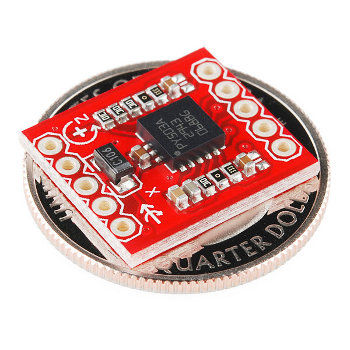
\includegraphics[width=0.3\linewidth]{img/giroscopio}
	\caption{Giroscopio}
	\label{fig:giroscopio}
\end{figure}

\addcontentsline{toc}{subsubsection}{Acelerómetro}
\subsection*{Acelerómetro}
\begin{itemize}
	\item \textbf{¿Qué mide?} La aceleración lineal en uno o más ejes (X, Y, Z) y puede detectar vibraciones, inclinaciones y fuerzas de impacto.
	\item \textbf{Principio de funcionamiento:} Basado en la segunda ley de Newton: F=maF = maF=ma.
	Los acelerómetros MEMS usan pequeñas masas móviles dentro del sensor que se desplazan con la aceleración, generando una señal eléctrica.
	\item \textbf{Aplicaciones:} Detección de caídas en dispositivos móviles y wearables.
	Control de movimiento en robots y videojuegos.
	Airbags en automóviles (detectan colisiones).
	Análisis de vibraciones en maquinaria industrial.
	\item \textbf{Ejemplo:} ADXL345 (digital, de 3 ejes).
	\cite{universalrobots_sensores_robótica}
	\cite{robotnik_sensores_2023}
\end{itemize}
\begin{figure}[h]
	\centering
	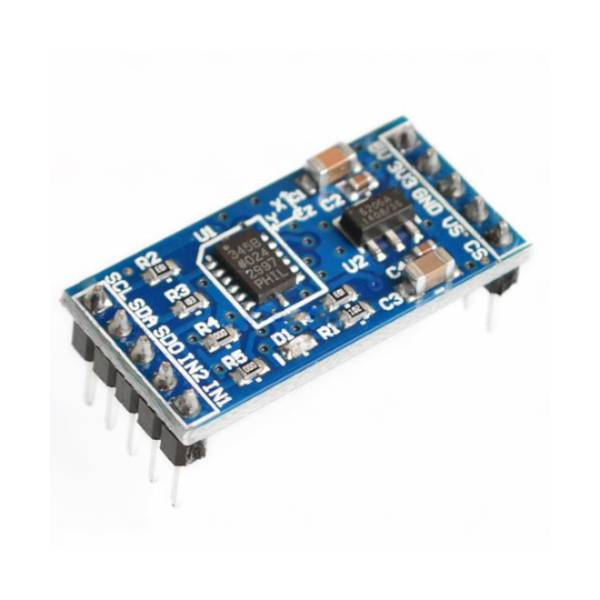
\includegraphics[width=0.3\linewidth]{img/acelerometro}
	\caption{Acelerometro}
	\label{fig:acelerometro}
\end{figure}

\addcontentsline{toc}{subsubsection}{Magnetómetro}
\subsection*{Magnetómetro}
\begin{itemize}
	\item \textbf{¿Qué mide?} La intensidad y dirección de los campos magnéticos y permite determinar la orientación respecto al campo magnético terrestre (como una brújula digital).
	\item \textbf{Principio de funcionamiento:} Utilizan el efecto Doppler: Utiliza el efecto Hall o materiales magnetorresistivos para detectar cambios en los campos magnéticos.
	Puede detectar objetos metálicos o variaciones en el campo magnético de la Tierra.
	\item \textbf{Aplicaciones:} Brújulas digitales en smartphones y GPS.
	Navegación en vehículos autónomos y drones.
	Detectores de metales.
	Exploración geofísica para medir anomalías magnéticas en la Tierra.
	\item \textbf{Ejemplo:} HMC5883L (popular en drones y navegación).
		\cite{makeblock_sensores_2025}
\end{itemize}
\begin{figure}[h]
	\centering
	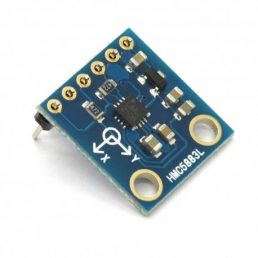
\includegraphics[width=0.3\linewidth]{img/magnetometro}
	\caption{Magnetómetro}
	\label{fig:magnetometro}
\end{figure}

\addcontentsline{toc}{subsubsection}{Light Detection and Ranging}
\subsection*{LiDAR (Light Detection and Ranging)}
\begin{itemize}
	\item \textbf{¿Qué mide?} Distancias a objetos mediante la emisión y recepción de pulsos láser.
	Puede generar mapas en 3D con alta precisión.
	\item \textbf{Principio de funcionamiento:}Emite un pulso de luz láser y mide el tiempo que tarda en reflejarse en un objeto y regresar al sensor.
	\item \textbf{Aplicaciones:} Vehículos autónomos (detección de obstáculos y mapeo).
	Topografía y cartografía en 3D.
	Agricultura de precisión (detección de variaciones en el terreno).
	Arqueología (descubrimiento de estructuras ocultas bajo vegetación).
	\item \textbf{Ejemplo:} Velodyne LiDAR (usado en coches autónomos).
	RPLIDAR A1 (más accesible para proyectos de robótica).
	\cite{yellowscan_lidar_2025}
\end{itemize}
\begin{figure}[h]
	\centering
	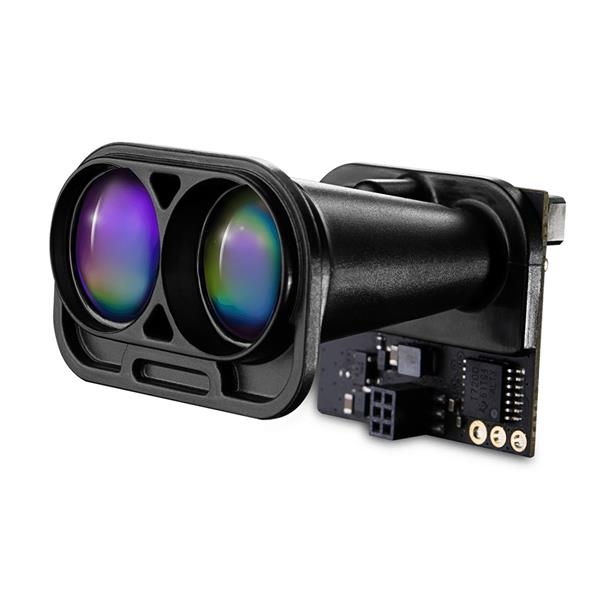
\includegraphics[width=0.3\linewidth]{img/LiDAR}
	\caption{LiDAR}
	\label{fig:LiDAR}
\end{figure}